\section{Le jeu de rôle, un renouveau de création populaire}

\begin{figure}[h!]
    \centering
    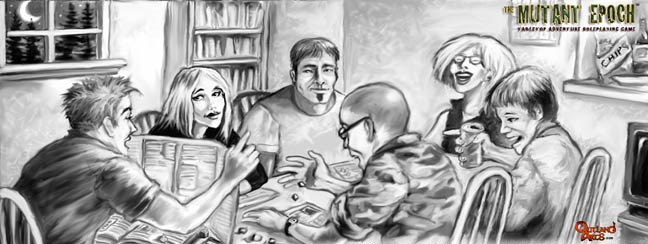
\includegraphics[width=0.85\linewidth]{img/rpg_tabletop1.jpg}
    \caption{Séance de jeu de rôle \textit{sur table}}
\end{figure}

\subsection{Le théâtre du social}

\begin{shadequote}
Le principe des jeux de rôle se rapproche davantage du théâtre improvisé que d'un jeu de société traditionnel. \par\emph{C{\'e}cile Cristofari \cite{cristofari2010lecteur}}
\end{shadequote}

Liant théâtre et jeu de société en une même entité, le jeu de rôle s'inspire des phénomènes d'imitation et d'identification observés sur scène et lors de l'écoute d'un récit. Si de nombreuses variantes du jeu de rôle existent, depuis les mises en scène pédagogiques jusqu'aux pratiques virtuelles, cet écrit limitera son champ d'étude au jeu de société éponyme. On parlera alors de jeu de rôle \textit{sur table}\footnote{Afin de limiter le contexte de cette étude, le terme \textit{jeu de rôle} utilisé dans la suite de cet écrit référencera exclusivement les jeux de rôle \textit{sur table}}, les seuls matériaux requis pour cette pratique étant un crayon, une feuille de papier, un set de dés et une table.\\

Il s'agît donc ici d'un style de jeu à travers lequel un ensemble de joueur(se)s incarnent un personnage évoluant dans un univers fictif ou inspiré du monde réel. On divisera alors la communauté de joueurs en deux types de rôles.

En premier lieu, le \textit{maître du jeu} est un joueur en charge du choix et  / ou de l'invention des règles et du monde dans lequel les autres joueurs évolueront. Il veille également au bon déroulement de l'histoire que leurs personnages vivront. Il lui incombe de décrire oralement l'environnement direct auquel les personnages font face dans le monde imaginaire de son choix, ce afin que les joueurs puissent accorder leur représentation du monde à la sienne. Il endosse également le rôle de guide, déclenchant et décrivant à sa convenance divers évènements dans ce même monde. Ces évènements, faisant appel aux réactions des joueurs, serviront essentiellement à guider les joueurs vers et à travers la trame chargée d'aventures que le \textit{maître du jeu} souhaite leur narrer. Il interprète enfin les rôles des personnages non joueurs présents dans son monde.

En second lieu, le reste de la communauté, usuellement composée de trois à six joueurs, interprète un personnage de son choix dans le monde décrit par le \textit{maître du jeu}. Les joueurs interagissent avec celui-ci ainsi qu'avec les autres personnages (joueurs et non joueurs) grâce à des descriptions orales de leurs actions, pouvant être accompagnées de mimes. Ils peuvent également endosser le rôle de leur personnage et s'exprimer comme tel à l'intention des autres personnages.

Il est ici important de noter la séparation marquée entre le monde réel où s'expriment les joueurs, et le monde imaginaire où s'expriment les personnages. Cette gestion de la profondeur du jeu représente un exercice mental sur lequel nous reviendrons.\\


L'histoire avec laquelle les joueurs interagissent ne connaît de limites que celles de l'imaginaire, de même que le monde et ses règles dans lesquels elle s'inscrit. Les joueurs peuvent être confrontés à des énigmes, des adversaires, des actions périlleuses dont l'issue dépendra du résultat d'un jet de dé, et tout doit être fait pour que l'expérience de jeu soit un plaisir pour la communauté. On notera la grande diversité des dés utilisés, le nombre de faces de ceux-ci variant de 4 à 20 en fonction du type de jet requis.

La durée des parties variant de quelques heures à plusieurs jours, celles-ci sont le plus souvent découpées en séances de jeu réparties dans le temps. On comprendra donc que le but de ce type jeu ne réside pas tant dans la victoire individuelle, mais plutôt dans l'accomplissement collectif des épreuves rencontrées et dans le plaisir pris dans le cadre de cette expérience imaginaire et sociale. La fin d'une partie sonnera enfin une fois l'objectif principal de l'histoire atteint, bien que celle-ci puisse être étendue si désiré.\\


\begin{figure}[h!]
    \centering
    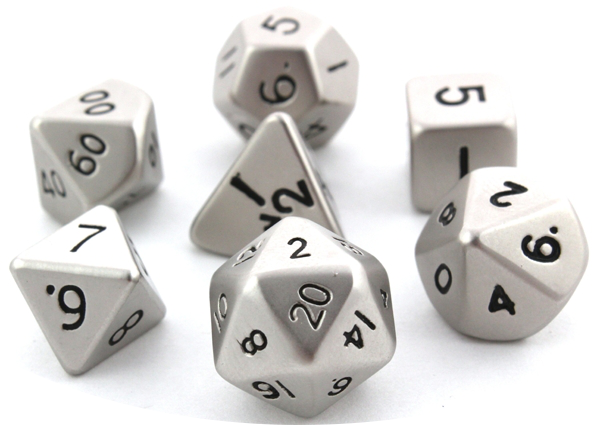
\includegraphics[width=0.80\linewidth]{img/dice_set.png}
    \caption{Set de dés utilisé pour les jeux de rôle}
\end{figure}

\clearpage


\subsection{L'expression de l'inconscient}

\begin{shadequote}
Le jeu de rôle [...] constitue un formidable outil visant à améliorer la communication, l'aisance sociale et la découverte de soi.
\par\emph{Anne-Marie Cariou-Rognant, Anne-Françoise Chaperon, Nicolas Duchesne, L'affirmation de soi par le jeu de rôle}
\end{shadequote}

Le jeu de rôle tel qu'ici décrit tirerait son origine des jeux de rôle thérapeutiques et psychanalytiques, élaborés dans les années 1920. Ce type de jeu est alors construit de manière à permettre l'exercice d'une \textit{catharsis}, amenant le patient à exprimer son \textit{Moi} intérieur, dans le but de libérer celui-ci de ses traumatismes affectifs refoulés. Il fut en effet observé que de tels jeux d'improvisation accompagnés de leur identification provoquaient un relâchement du processus de \textit{censure} du patient, permettant une certaine appréhension de son inconscient par le psychanalyste. Cette technique est nommé \textit{psychodrame analytique}.

En d'autres termes, les jeux de rôle sont considérés dans le domaine de la psychanalyse comme une aire d'expérience où les réactions de l'individu, partiellement libérées des normes sociales, peuvent être analysées. Ces jeux peuvent en effet être le lieu de réalisation de fantasmes et évènements socialement inacceptables dans le monde réel.\\


L'efficacité d'une telle méthode ne peut par ailleurs qu'être constatée lorsque l'on étudie le choix de représentation des patients dans ce monde imaginaire. Ceux-ci tendent en effet à s'idéaliser à travers leur personnage, afin d'obtenir en cet univers une place qui leur est refusée dans le monde réel. L'interprétation d'une personnalité opposée peut également s'observer, tel lorsqu'un patient atteint d'une forte timidité simule une personnalité extravertie.

L'exercice du jeu de rôle est alors élevé au rang de pratique thérapeutique, clé de la découverte de l'individu, permettant en outre à un joueur de prendre confiance en lui par l'exercice des compétences qui lui font défaut.



\subsection{Une communauté captive}

\begin{shadequote}
[...] il est important de s’identifier à un personnage qui permet de mettre en scène les désirs que le canon laisse insatisfaits [...]
\par\emph{C{\'e}cile Cristofari}
\end{shadequote}

Occupant une place centrale dans le jeu de rôle, l'identification d'un joueur à son personnage serait une des raisons clefs de la captivité de cette communauté. L'attache sentimentale à ce personnage fictif pourrait même revêtir davantage d'importance que l'histoire vécue, et causer une forte addiction d'un acabit comparable à celui observé dans le domaine des jeux vidéos. \`A un stade fort évolué, cette addiction se caractérise par un désintérêt du monde réel au profit de la vie fictive, libérée et trépidante, dont le joueur fait l'expérience.\\


Selon Olivier Caïra\cite{caira2007jeux}, cet attrait proviendrait de la multitude et de la complexité des compétences requises par ce mode de jeu. Outre la cohabitation entre les rôles de \textit{maître du jeu} et joueur \textit{lambda}, l'exercice mental de représentation du niveau de jeu (monde réel ou imaginaire) doit s'accompagner d'une variation de la communication et du registre de langue utilisé entre les joueurs. Ce registre doit être fonction du degré de profondeur du jeu, selon qu'il s'agît de descriptions du monde ou d'actions, de commentaires destinés aux joueurs ou de dialogues entre personnages. La notion de communication en aparté doit également être prise en compte, une pratique adaptée de ces éléments couplée à une ambiance de jeu adéquate favorisant une immersion maximale dans le monde imaginé.

On notera par ailleurs l'équilibre requis au sein d'une équipe de personnages, ceux-ci devant disposer de rôles complémentaires afin de réagir efficacement aux évènements rencontrés. Si chaque personnage créé se voit assigner un certain niveau par domaine de compétences, le jeu de scène du joueur ne doit pas être oublié, lequel améliore ses propres compétences en les pratiquant (cohésion de groupe, éloquence, stratégie...).\\


Un dernier facteur d'attrait pour une communauté réside dans l'univers visé. De nombreux univers et scénarios ont une origine littéraire ou cinématographiques, tels l'\textit{Appel de Cthulhu} de Lovecraft, \textit{Le seigneur des anneaux} de Tolkien ou encore \textit{Star Wars} de George Lucas, chacune de ces \oe uvres ayant donné naissance à un monde dans lequel une communauté passionnée développa rapidement des règles de jeu et scénarios. La fidélité vis-à-vis de l'\oe uvre originelle est alors libre au \textit{maître du jeu}, de nombreux jeux de rôle étendant le monde et l'intrigue de la fiction originelle.

\clearpage
